\begin{frame}
\end{frame}

\begin{frame}
  \frametitle{授课教材}
  \begin{figure}
    \centering
    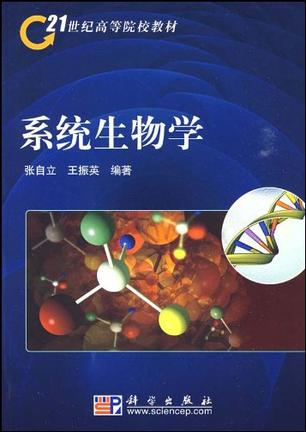
\includegraphics[width=5cm]{c0.book.jpg}
  \end{figure}
\end{frame}

\begin{frame}
  \frametitle{课程安排 | 理论课}
  \begin{table}
    \centering
    \rowcolors[]{1}{blue!20}{blue!10}
    \begin{tabular}{cllcc}
      \hline
      \rowcolor{blue!50}顺序 & 授课内容 & 教材章节 & 学时 & 授课教师\\
      \hline
      1 & 概论 & 第1章 & 2 & 伊现富\\
      2 & 基因组学 & 第2章 & 6 & 伊现富\\
      3 & 转录组学 & 第3章 & 6 & 伊现富\\
      4 &  & 第4章 & 2 & \\
      5 &  & 第5章 & 2 & \\
      6 &  & 第6章 & 2 & \\
      7 &  & 第7章 & 2 & \\
      8 &  & 第8章 & 2 & \\
      9 &  & 第9章 & 2 & \\
      \hline
    \end{tabular}
  \end{table}
\end{frame}

\begin{frame}
  \frametitle{课程安排 | 实验课}
  \begin{table}
    \centering
    \rowcolors[]{1}{blue!20}{blue!10}
    \begin{tabular}{cllcc}
      \hline
      \rowcolor{blue!50}顺序 & 实验内容 & 理论知识 & 学时 & 授课教师\\
      1 & 外线组测序数据分析 & 基因组 & 3 & 伊现富\\
      2 & 转录组测序数据分析 & 转录组 & 3 & 伊现富\\
      3 & & & 3 & \\
      4 & & & 3 & \\
      5 & & & 3 & \\
      6 & & & 3 & \\
      \hline
    \end{tabular}
  \end{table}
\end{frame}

\begin{frame}
  \frametitle{考核方式}
  \begin{enumerate}
    \item 理论课:50\%
      \begin{enumerate}
        \item 平时表现:10\%
        \item 闭卷考试:40\%
      \end{enumerate}
    \item 实验课:30\%
      \begin{enumerate}
        \item 平时表现:10\%
        \item 实验报告:20\%
      \end{enumerate}
    \item 课堂讨论:20\%
      \begin{enumerate}
        \item 报告答辩:10\%
        \item 报告论文:10\%
      \end{enumerate}
  \end{enumerate}
\end{frame}

